\documentclass[]{article}
\usepackage{lmodern}
\usepackage{amssymb,amsmath}
\usepackage{ifxetex,ifluatex}
\usepackage{fixltx2e} % provides \textsubscript
\ifnum 0\ifxetex 1\fi\ifluatex 1\fi=0 % if pdftex
  \usepackage[T1]{fontenc}
  \usepackage[utf8]{inputenc}
\else % if luatex or xelatex
  \ifxetex
    \usepackage{mathspec}
  \else
    \usepackage{fontspec}
  \fi
  \defaultfontfeatures{Ligatures=TeX,Scale=MatchLowercase}
\fi
% use upquote if available, for straight quotes in verbatim environments
\IfFileExists{upquote.sty}{\usepackage{upquote}}{}
% use microtype if available
\IfFileExists{microtype.sty}{%
\usepackage{microtype}
\UseMicrotypeSet[protrusion]{basicmath} % disable protrusion for tt fonts
}{}
\usepackage[margin=1in]{geometry}
\usepackage{hyperref}
\hypersetup{unicode=true,
            pdftitle={BEES3041: Modelling the photosynthetic response to environmental conditions},
            pdfborder={0 0 0},
            breaklinks=true}
\urlstyle{same}  % don't use monospace font for urls
\usepackage{color}
\usepackage{fancyvrb}
\newcommand{\VerbBar}{|}
\newcommand{\VERB}{\Verb[commandchars=\\\{\}]}
\DefineVerbatimEnvironment{Highlighting}{Verbatim}{commandchars=\\\{\}}
% Add ',fontsize=\small' for more characters per line
\usepackage{framed}
\definecolor{shadecolor}{RGB}{248,248,248}
\newenvironment{Shaded}{\begin{snugshade}}{\end{snugshade}}
\newcommand{\AlertTok}[1]{\textcolor[rgb]{0.94,0.16,0.16}{#1}}
\newcommand{\AnnotationTok}[1]{\textcolor[rgb]{0.56,0.35,0.01}{\textbf{\textit{#1}}}}
\newcommand{\AttributeTok}[1]{\textcolor[rgb]{0.77,0.63,0.00}{#1}}
\newcommand{\BaseNTok}[1]{\textcolor[rgb]{0.00,0.00,0.81}{#1}}
\newcommand{\BuiltInTok}[1]{#1}
\newcommand{\CharTok}[1]{\textcolor[rgb]{0.31,0.60,0.02}{#1}}
\newcommand{\CommentTok}[1]{\textcolor[rgb]{0.56,0.35,0.01}{\textit{#1}}}
\newcommand{\CommentVarTok}[1]{\textcolor[rgb]{0.56,0.35,0.01}{\textbf{\textit{#1}}}}
\newcommand{\ConstantTok}[1]{\textcolor[rgb]{0.00,0.00,0.00}{#1}}
\newcommand{\ControlFlowTok}[1]{\textcolor[rgb]{0.13,0.29,0.53}{\textbf{#1}}}
\newcommand{\DataTypeTok}[1]{\textcolor[rgb]{0.13,0.29,0.53}{#1}}
\newcommand{\DecValTok}[1]{\textcolor[rgb]{0.00,0.00,0.81}{#1}}
\newcommand{\DocumentationTok}[1]{\textcolor[rgb]{0.56,0.35,0.01}{\textbf{\textit{#1}}}}
\newcommand{\ErrorTok}[1]{\textcolor[rgb]{0.64,0.00,0.00}{\textbf{#1}}}
\newcommand{\ExtensionTok}[1]{#1}
\newcommand{\FloatTok}[1]{\textcolor[rgb]{0.00,0.00,0.81}{#1}}
\newcommand{\FunctionTok}[1]{\textcolor[rgb]{0.00,0.00,0.00}{#1}}
\newcommand{\ImportTok}[1]{#1}
\newcommand{\InformationTok}[1]{\textcolor[rgb]{0.56,0.35,0.01}{\textbf{\textit{#1}}}}
\newcommand{\KeywordTok}[1]{\textcolor[rgb]{0.13,0.29,0.53}{\textbf{#1}}}
\newcommand{\NormalTok}[1]{#1}
\newcommand{\OperatorTok}[1]{\textcolor[rgb]{0.81,0.36,0.00}{\textbf{#1}}}
\newcommand{\OtherTok}[1]{\textcolor[rgb]{0.56,0.35,0.01}{#1}}
\newcommand{\PreprocessorTok}[1]{\textcolor[rgb]{0.56,0.35,0.01}{\textit{#1}}}
\newcommand{\RegionMarkerTok}[1]{#1}
\newcommand{\SpecialCharTok}[1]{\textcolor[rgb]{0.00,0.00,0.00}{#1}}
\newcommand{\SpecialStringTok}[1]{\textcolor[rgb]{0.31,0.60,0.02}{#1}}
\newcommand{\StringTok}[1]{\textcolor[rgb]{0.31,0.60,0.02}{#1}}
\newcommand{\VariableTok}[1]{\textcolor[rgb]{0.00,0.00,0.00}{#1}}
\newcommand{\VerbatimStringTok}[1]{\textcolor[rgb]{0.31,0.60,0.02}{#1}}
\newcommand{\WarningTok}[1]{\textcolor[rgb]{0.56,0.35,0.01}{\textbf{\textit{#1}}}}
\usepackage{graphicx,grffile}
\makeatletter
\def\maxwidth{\ifdim\Gin@nat@width>\linewidth\linewidth\else\Gin@nat@width\fi}
\def\maxheight{\ifdim\Gin@nat@height>\textheight\textheight\else\Gin@nat@height\fi}
\makeatother
% Scale images if necessary, so that they will not overflow the page
% margins by default, and it is still possible to overwrite the defaults
% using explicit options in \includegraphics[width, height, ...]{}
\setkeys{Gin}{width=\maxwidth,height=\maxheight,keepaspectratio}
\IfFileExists{parskip.sty}{%
\usepackage{parskip}
}{% else
\setlength{\parindent}{0pt}
\setlength{\parskip}{6pt plus 2pt minus 1pt}
}
\setlength{\emergencystretch}{3em}  % prevent overfull lines
\providecommand{\tightlist}{%
  \setlength{\itemsep}{0pt}\setlength{\parskip}{0pt}}
\setcounter{secnumdepth}{0}
% Redefines (sub)paragraphs to behave more like sections
\ifx\paragraph\undefined\else
\let\oldparagraph\paragraph
\renewcommand{\paragraph}[1]{\oldparagraph{#1}\mbox{}}
\fi
\ifx\subparagraph\undefined\else
\let\oldsubparagraph\subparagraph
\renewcommand{\subparagraph}[1]{\oldsubparagraph{#1}\mbox{}}
\fi

%%% Use protect on footnotes to avoid problems with footnotes in titles
\let\rmarkdownfootnote\footnote%
\def\footnote{\protect\rmarkdownfootnote}

%%% Change title format to be more compact
\usepackage{titling}

% Create subtitle command for use in maketitle
\newcommand{\subtitle}[1]{
  \posttitle{
    \begin{center}\large#1\end{center}
    }
}

\setlength{\droptitle}{-2em}

  \title{BEES3041: Modelling the photosynthetic response to environmental
conditions}
    \pretitle{\vspace{\droptitle}\centering\huge}
  \posttitle{\par}
    \author{}
    \preauthor{}\postauthor{}
    \date{}
    \predate{}\postdate{}
  

\begin{document}
\maketitle


\includegraphics[width=0.3\linewidth]{data/logo}

\hypertarget{introduction}{%
\section{Introduction}\label{introduction}}

In this lab we are going to explore the C\textsubscript{3} leaf-level
photosynthesis model proposed by Farquhar, Caemmerer, and Berry (1980)
and use this to simulate photosynthesis at leaf, ecosystem and global
scales. The model is central to all land schemes embedded in
coupled-climate models and predicts that photosynthesis is limited by
the slowest of three biochemical processes:

\begin{enumerate}
\def\labelenumi{\arabic{enumi}.}
\tightlist
\item
  Maximum rate of Rubisco-catalysed carboxylation
\item
  Rate of ribulose 1,5-bisphosphate (RuBP) regeneration via electron
  transport
\item
  The rate of RuBP regeneration via triose phosphate utilisation
\end{enumerate}

In this practical we are only going to consider the first two
limitations. There a number of great papers which cover this subject in
detail, see for example, Bernacchi et al. (2013), Medlyn et al. (2002)
and Sharkey (1985).

We are going to use this model to:

\begin{itemize}
\tightlist
\item
  learn how leaf-level photosynthesis responds to changes in the
  environmental forcing (photosynthetically active radiation,
  temperature and carbon dioxide).
\item
  simulate GPP at the ecosystem-scale (\textasciitilde{}1 km\^{}2) using
  FLUXNET (eddy covariance) meteorological data.
\item
  simulate a global estimate of GPP.
\end{itemize}

From playing with this model across scales, we should start to see the
key assumptions that our model makes. We should also begin to identify
the key weakness in our approach as we apply the model at different
scales.

\begin{center}\rule{0.5\linewidth}{\linethickness}\end{center}

\hypertarget{temperature-responses-of-model-parameters}{%
\section{Temperature responses of model
parameters}\label{temperature-responses-of-model-parameters}}

Let's start by exploring the response of the model to temperature. First
we need to generate some temperature data:

\begin{Shaded}
\begin{Highlighting}[]
\KeywordTok{library}\NormalTok{(ggplot2)}

\KeywordTok{source}\NormalTok{(}\StringTok{"R/photosynthesis.R"}\NormalTok{)}
\KeywordTok{source}\NormalTok{(}\StringTok{"R/parameters.R"}\NormalTok{)}
\KeywordTok{source}\NormalTok{(}\StringTok{"R/constants.R"}\NormalTok{)}

\NormalTok{Tleaf <-}\StringTok{ }\KeywordTok{seq}\NormalTok{(}\FloatTok{0.0}\NormalTok{, }\FloatTok{50.0}\NormalTok{, }\FloatTok{0.5}\NormalTok{) }\OperatorTok{+}\StringTok{ }\NormalTok{DEG_}\DecValTok{2}\NormalTok{_KELVIN}
\end{Highlighting}
\end{Shaded}

The photosynthesis model has two major parameters, the potential rate of
electron transport (Jmax) and the maximum rate of Rubisco activity
(Vcmax). Both of these parameters vary as a function of temperature,
let's plot them. I've copied the function calls from photosynthes.R:

\begin{Shaded}
\begin{Highlighting}[]
\NormalTok{Vcmax <-}\StringTok{ }\KeywordTok{peaked_arrh}\NormalTok{(p}\OperatorTok{$}\NormalTok{Vcmax25, p}\OperatorTok{$}\NormalTok{Eav, Tleaf, p}\OperatorTok{$}\NormalTok{deltaSv, p}\OperatorTok{$}\NormalTok{Hdv)}
\NormalTok{Jmax <-}\StringTok{ }\KeywordTok{peaked_arrh}\NormalTok{(p}\OperatorTok{$}\NormalTok{Jmax25, p}\OperatorTok{$}\NormalTok{Eaj, Tleaf, p}\OperatorTok{$}\NormalTok{deltaSj, p}\OperatorTok{$}\NormalTok{Hdj)}

\NormalTok{df <-}\StringTok{ }\KeywordTok{data.frame}\NormalTok{(Tleaf, Vcmax, Jmax)}

\KeywordTok{ggplot}\NormalTok{(df, }\KeywordTok{aes}\NormalTok{(Tleaf}\OperatorTok{-}\NormalTok{DEG_}\DecValTok{2}\NormalTok{_KELVIN)) }\OperatorTok{+}
\StringTok{  }\KeywordTok{geom_line}\NormalTok{(}\KeywordTok{aes}\NormalTok{(}\DataTypeTok{y=}\NormalTok{Vcmax, }\DataTypeTok{colour=}\StringTok{"Vcmax"}\NormalTok{)) }\OperatorTok{+}
\StringTok{  }\KeywordTok{geom_line}\NormalTok{(}\KeywordTok{aes}\NormalTok{(}\DataTypeTok{y=}\NormalTok{Jmax, }\DataTypeTok{colour=}\StringTok{"Jmax"}\NormalTok{)) }\OperatorTok{+}
\StringTok{  }\KeywordTok{ylab}\NormalTok{(}\KeywordTok{expression}\NormalTok{(}\StringTok{"Paramater"} \OperatorTok{~}\StringTok{ }\NormalTok{(mu }\OperatorTok{*}\StringTok{ }\NormalTok{mol }\OperatorTok{~}\StringTok{  }\NormalTok{m}\OperatorTok{^}\NormalTok{\{}\OperatorTok{-}\DecValTok{2}\NormalTok{\}  }\OperatorTok{~}\StringTok{  }\NormalTok{s}\OperatorTok{^}\NormalTok{\{}\OperatorTok{-}\DecValTok{1}\NormalTok{\}))) }\OperatorTok{+}
\StringTok{  }\KeywordTok{xlab}\NormalTok{(}\KeywordTok{expression}\NormalTok{(}\StringTok{'Temperature ('}\OperatorTok{*}\ErrorTok{~}\NormalTok{degree}\OperatorTok{*}\NormalTok{C}\OperatorTok{*}\StringTok{')'}\NormalTok{)) }\OperatorTok{+}\StringTok{ }
\StringTok{  }\KeywordTok{theme_classic}\NormalTok{() }\OperatorTok{+}
\StringTok{  }\KeywordTok{theme}\NormalTok{(}\DataTypeTok{legend.title=}\KeywordTok{element_blank}\NormalTok{()) }\OperatorTok{+}
\StringTok{  }\KeywordTok{scale_colour_brewer}\NormalTok{(}\DataTypeTok{palette =} \StringTok{"Set2"}\NormalTok{)}
\end{Highlighting}
\end{Shaded}

\includegraphics{BEES3041_lab_files/figure-latex/unnamed-chunk-2-1.pdf}

In the model both parameters are modelled using a peaked form of the
Arrhenius equation. The Eav/Eaj parameters give the exponential increase
of the function below the optimum; the Hdv/Hdj parameters describe the
rate of decrease of the function above the optimum.

Let's see what values we used:

\begin{Shaded}
\begin{Highlighting}[]
\KeywordTok{print}\NormalTok{(}\KeywordTok{c}\NormalTok{(p}\OperatorTok{$}\NormalTok{Vcmax25, p}\OperatorTok{$}\NormalTok{Eav, p}\OperatorTok{$}\NormalTok{deltaSv, p}\OperatorTok{$}\NormalTok{Hdv))}
\end{Highlighting}
\end{Shaded}

\begin{verbatim}
## [1]     40.00  51560.00    629.26 200000.00
\end{verbatim}

\begin{Shaded}
\begin{Highlighting}[]
\KeywordTok{print}\NormalTok{(}\KeywordTok{c}\NormalTok{(p}\OperatorTok{$}\NormalTok{Jmax25, p}\OperatorTok{$}\NormalTok{Eaj, p}\OperatorTok{$}\NormalTok{deltaSj, p}\OperatorTok{$}\NormalTok{Hdj))}
\end{Highlighting}
\end{Shaded}

\begin{verbatim}
## [1]     66.8000  43790.0000    644.4338 200000.0000
\end{verbatim}

Let's tweak these values and see how our functions respond to
temperature

\begin{Shaded}
\begin{Highlighting}[]
\NormalTok{Vcmax <-}\StringTok{ }\KeywordTok{peaked_arrh}\NormalTok{(p}\OperatorTok{$}\NormalTok{Vcmax25, p}\OperatorTok{$}\NormalTok{Eav, Tleaf, p}\OperatorTok{$}\NormalTok{deltaSv, p}\OperatorTok{$}\NormalTok{Hdv)}
\NormalTok{Vcmax2 <-}\StringTok{ }\KeywordTok{peaked_arrh}\NormalTok{(p}\OperatorTok{$}\NormalTok{Vcmax25, }\DecValTok{40000}\NormalTok{, Tleaf, }\FloatTok{620.0}\NormalTok{, p}\OperatorTok{$}\NormalTok{Hdv)}
\NormalTok{Vcmax3 <-}\StringTok{ }\KeywordTok{peaked_arrh}\NormalTok{(p}\OperatorTok{$}\NormalTok{Vcmax25, }\DecValTok{70000}\NormalTok{, Tleaf, }\FloatTok{650.0}\NormalTok{, p}\OperatorTok{$}\NormalTok{Hdv)}


\NormalTok{df <-}\StringTok{ }\KeywordTok{data.frame}\NormalTok{(Tleaf, Vcmax, Jmax)}

\KeywordTok{ggplot}\NormalTok{(df, }\KeywordTok{aes}\NormalTok{(Tleaf}\OperatorTok{-}\NormalTok{DEG_}\DecValTok{2}\NormalTok{_KELVIN)) }\OperatorTok{+}
\StringTok{  }\KeywordTok{geom_line}\NormalTok{(}\KeywordTok{aes}\NormalTok{(}\DataTypeTok{y=}\NormalTok{Vcmax, }\DataTypeTok{colour=}\StringTok{"Vcmax"}\NormalTok{)) }\OperatorTok{+}
\StringTok{  }\KeywordTok{geom_line}\NormalTok{(}\KeywordTok{aes}\NormalTok{(}\DataTypeTok{y=}\NormalTok{Vcmax2, }\DataTypeTok{colour=}\StringTok{"Vcmax2"}\NormalTok{)) }\OperatorTok{+}
\StringTok{  }\KeywordTok{geom_line}\NormalTok{(}\KeywordTok{aes}\NormalTok{(}\DataTypeTok{y=}\NormalTok{Vcmax3, }\DataTypeTok{colour=}\StringTok{"Vcmax3"}\NormalTok{)) }\OperatorTok{+}
\StringTok{  }\KeywordTok{ylab}\NormalTok{(}\KeywordTok{expression}\NormalTok{(}\StringTok{"Vcmax"} \OperatorTok{~}\StringTok{ }\NormalTok{(mu }\OperatorTok{*}\StringTok{ }\NormalTok{mol }\OperatorTok{~}\StringTok{  }\NormalTok{m}\OperatorTok{^}\NormalTok{\{}\OperatorTok{-}\DecValTok{2}\NormalTok{\}  }\OperatorTok{~}\StringTok{  }\NormalTok{s}\OperatorTok{^}\NormalTok{\{}\OperatorTok{-}\DecValTok{1}\NormalTok{\}))) }\OperatorTok{+}
\StringTok{  }\KeywordTok{xlab}\NormalTok{(}\KeywordTok{expression}\NormalTok{(}\StringTok{'Temperature ('}\OperatorTok{*}\ErrorTok{~}\NormalTok{degree}\OperatorTok{*}\NormalTok{C}\OperatorTok{*}\StringTok{')'}\NormalTok{)) }\OperatorTok{+}\StringTok{ }
\StringTok{  }\KeywordTok{theme_classic}\NormalTok{() }\OperatorTok{+}
\StringTok{  }\KeywordTok{theme}\NormalTok{(}\DataTypeTok{legend.title=}\KeywordTok{element_blank}\NormalTok{()) }\OperatorTok{+}
\StringTok{  }\KeywordTok{scale_colour_brewer}\NormalTok{(}\DataTypeTok{palette =} \StringTok{"Set2"}\NormalTok{)}
\end{Highlighting}
\end{Shaded}

\includegraphics{BEES3041_lab_files/figure-latex/unnamed-chunk-4-1.pdf}

In the model, the Rubisco-limited photosynthesis rate is made up of five
paramaters:

\begin{enumerate}
\def\labelenumi{\arabic{enumi}.}
\tightlist
\item
  \(\Gamma\)\(^{*}\): the CO\textsubscript{2} compensation point in the
  absence of mitochondrial respiration.
\item
  V\textsubscript{cmax}: the maximum rate of Rubisco activity.
\item
  R\textsubscript{d}: leaf mitochondrial respiration in the light (day
  respiration).
\item
  K\textsubscript{o}: Michaelis-- Menten coefficients for oxygenation.
\item
  K\textsubscript{c}: Michaelis-- Menten coefficients for carboxylation.
\end{enumerate}

Each of these parameters is temperature dependent, thus the skill of the
model depends on correctly accounting for these response to temperature
when using the model. When we use these model parameters in global
models we typical assume that the parameters (excluding
V\textsubscript{cmax}) are conserved across species. This assumption is
broadly supported by observations, but what do we think happens in
different growing conditions? By contrast, leaf measurements suggest
that V\textsubscript{cmax} varies considerably: varying between leaves
within a single plant, across growing seasons and across plants. In
global models, we typically assume that we can represent this
variability using 5-11 plant functional types, see Rogers, A. Photosynth
Res (2014) 119: 15. \url{https://doi.org/10.1007/s11120-013-9818-1} for
more details. Even when we do this in models, the disagreement across
models is striking.

\begin{center}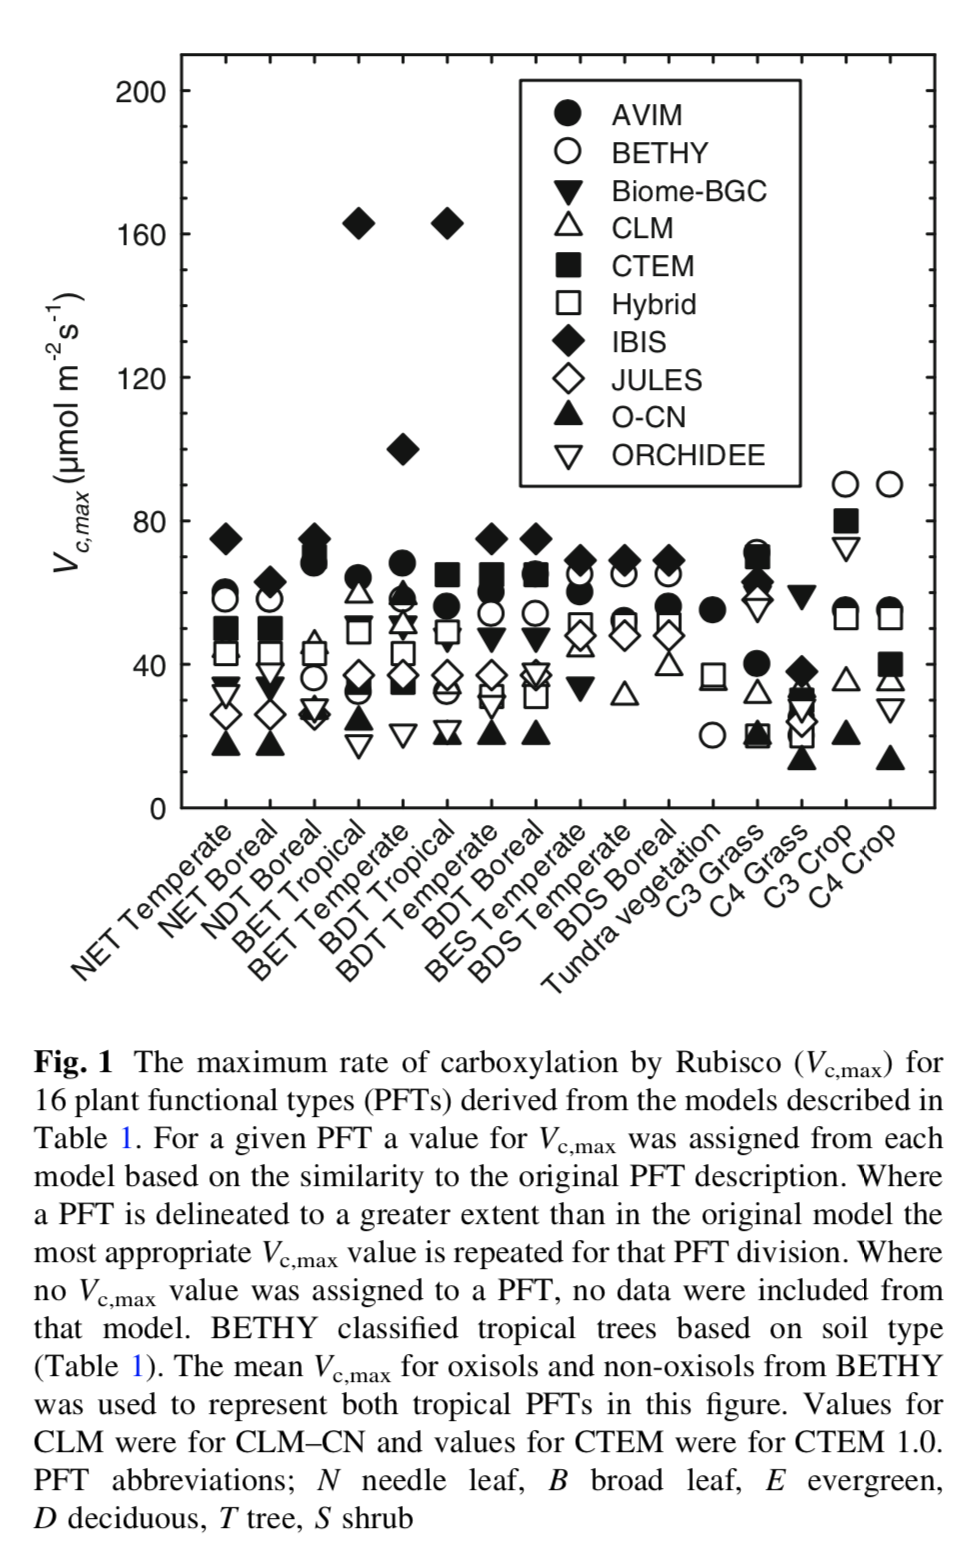
\includegraphics[width=0.4\linewidth]{data/rogers} \end{center}

Now that you've seen how to call the functions to calculate
V\textsubscript{cmax} and J\textsubscript{max}, can you look in the code
(R/photosynthesis.R) and also plot \(\Gamma\)\(^{*}\),
R\textsubscript{d}m, K\textsubscript{o} and K\textsubscript{m} as a
function of temperature?

\begin{center}\rule{0.5\linewidth}{\linethickness}\end{center}

\hypertarget{response-to-temperature}{%
\section{Response to temperature}\label{response-to-temperature}}

From this understanding of how the key model parameters change with
temperature, can we make a prediction about how the rate of
photosynthesis is likely to change with temperature?

Let's make a plot to see if our predictions matched the models\ldots{}

\begin{Shaded}
\begin{Highlighting}[]
\NormalTok{Tleaf <-}\StringTok{ }\KeywordTok{seq}\NormalTok{(}\DecValTok{0}\NormalTok{, }\FloatTok{50.0}\NormalTok{, }\FloatTok{0.5}\NormalTok{) }\OperatorTok{+}\StringTok{ }\NormalTok{DEG_}\DecValTok{2}\NormalTok{_KELVIN}
\NormalTok{PAR <-}\StringTok{ }\FloatTok{1800.0}
\NormalTok{Cs <-}\StringTok{ }\FloatTok{400.0}
\NormalTok{vpd <-}\StringTok{ }\FloatTok{1.5}

\NormalTok{out <-}\StringTok{ }\KeywordTok{calc_photosynthesis}\NormalTok{(p, Tleaf, PAR, Cs, vpd, }\DataTypeTok{peaked_Vcmax=}\OtherTok{TRUE}\NormalTok{,}
                           \DataTypeTok{peaked_Jmax=}\OtherTok{TRUE}\NormalTok{)}
\NormalTok{df <-}\StringTok{ }\KeywordTok{data.frame}\NormalTok{(Tleaf, out}\OperatorTok{$}\NormalTok{An, out}\OperatorTok{$}\NormalTok{Ac, out}\OperatorTok{$}\NormalTok{Aj)}

\KeywordTok{ggplot}\NormalTok{(df, }\KeywordTok{aes}\NormalTok{(Tleaf}\OperatorTok{-}\NormalTok{DEG_}\DecValTok{2}\NormalTok{_KELVIN)) }\OperatorTok{+}
\StringTok{  }\KeywordTok{geom_line}\NormalTok{(}\KeywordTok{aes}\NormalTok{(}\DataTypeTok{y=}\NormalTok{out.Ac, }\DataTypeTok{colour=}\StringTok{"Rubisco-limited (Ac)"}\NormalTok{)) }\OperatorTok{+}
\StringTok{  }\KeywordTok{geom_line}\NormalTok{(}\KeywordTok{aes}\NormalTok{(}\DataTypeTok{y=}\NormalTok{out.Aj, }\DataTypeTok{colour=}\StringTok{"RuBP-limited (Aj)"}\NormalTok{)) }\OperatorTok{+}
\StringTok{  }\KeywordTok{ylab}\NormalTok{(}\KeywordTok{expression}\NormalTok{(}\StringTok{"Photosynthesis"} \OperatorTok{~}\StringTok{ }\NormalTok{(mu }\OperatorTok{*}\StringTok{ }\NormalTok{mol }\OperatorTok{~}\StringTok{  }\NormalTok{m}\OperatorTok{^}\NormalTok{\{}\OperatorTok{-}\DecValTok{2}\NormalTok{\}  }\OperatorTok{~}\StringTok{  }\NormalTok{s}\OperatorTok{^}\NormalTok{\{}\OperatorTok{-}\DecValTok{1}\NormalTok{\}))) }\OperatorTok{+}
\StringTok{  }\KeywordTok{xlab}\NormalTok{(}\KeywordTok{expression}\NormalTok{(}\StringTok{'Temperature ('}\OperatorTok{*}\ErrorTok{~}\NormalTok{degree}\OperatorTok{*}\NormalTok{C}\OperatorTok{*}\StringTok{')'}\NormalTok{)) }\OperatorTok{+}\StringTok{ }
\StringTok{  }\CommentTok{#theme_classic(base_size=16) +}
\StringTok{  }\KeywordTok{theme_classic}\NormalTok{() }\OperatorTok{+}
\StringTok{  }\KeywordTok{theme}\NormalTok{(}\DataTypeTok{legend.title=}\KeywordTok{element_blank}\NormalTok{()) }\OperatorTok{+}
\StringTok{  }\KeywordTok{theme}\NormalTok{(}\DataTypeTok{legend.position =} \KeywordTok{c}\NormalTok{(}\FloatTok{0.9}\NormalTok{, }\FloatTok{0.9}\NormalTok{)) }\OperatorTok{+}
\StringTok{  }\KeywordTok{scale_colour_brewer}\NormalTok{(}\DataTypeTok{palette =} \StringTok{"Set2"}\NormalTok{)}
\end{Highlighting}
\end{Shaded}

\includegraphics{BEES3041_lab_files/figure-latex/unnamed-chunk-5-1.pdf}

\begin{Shaded}
\begin{Highlighting}[]
\CommentTok{#if (dir.exists("plots") == FALSE) \{}
\CommentTok{#  dir.create("plots")}
\CommentTok{#\}}
\CommentTok{#ggsave("plots/Ac_Aj_temp.pdf", width=9, height=6) }
\end{Highlighting}
\end{Shaded}

The plot shows the response of A to temperature increases steadily until
it reaches an optimum point (T\textsubscript{opt}), after which A
declines at a faster rate.

The model assumes that the Rubisco-limited assimilation rate follows a
Michaelis--Menten response function, accounting for a competitive
inhibitor, oxygen. With Michaelis-Menten reactions, increasing the
limiting substrate, CO\textsubscript{2}, the amount of enzyme present,
Rubisco, or decreasing the competitive inhibitor, O2, will yield higher
reaction rates. The model also assumes that the RuBP
regeneration-limited rate of assimilation depends on the rate at which
the light reactions generate ATP and NADPH; this process is limited at
low light intensity.

Let's demonstrate this is the case by reducing and increasing the
intercellular concentration of O2 parameter and plotting the impact.
Rubisco catalyses the oxygenation of RuBP as well as carboxylation,
although the affinity for oxygen is lower than that for
CO\textsubscript{2}.

\begin{Shaded}
\begin{Highlighting}[]
\NormalTok{Tleaf <-}\StringTok{ }\KeywordTok{seq}\NormalTok{(}\DecValTok{0}\NormalTok{, }\FloatTok{50.0}\NormalTok{, }\FloatTok{0.5}\NormalTok{) }\OperatorTok{+}\StringTok{ }\NormalTok{DEG_}\DecValTok{2}\NormalTok{_KELVIN}
\NormalTok{PAR <-}\StringTok{ }\FloatTok{1800.0}
\NormalTok{Cs <-}\StringTok{ }\FloatTok{400.0}
\NormalTok{vpd <-}\StringTok{ }\FloatTok{1.5}

\NormalTok{p}\OperatorTok{$}\NormalTok{Oi =}\StringTok{ }\FloatTok{210.0}
\NormalTok{out_std <-}\StringTok{ }\KeywordTok{calc_photosynthesis}\NormalTok{(p, Tleaf, PAR, Cs, vpd, }\DataTypeTok{peaked_Vcmax=}\OtherTok{TRUE}\NormalTok{,}
                               \DataTypeTok{peaked_Jmax=}\OtherTok{TRUE}\NormalTok{)}

\NormalTok{p}\OperatorTok{$}\NormalTok{Oi =}\StringTok{ }\FloatTok{150.0}
\NormalTok{out_low <-}\StringTok{ }\KeywordTok{calc_photosynthesis}\NormalTok{(p, Tleaf, PAR, Cs, vpd, }\DataTypeTok{peaked_Vcmax=}\OtherTok{TRUE}\NormalTok{,}
                               \DataTypeTok{peaked_Jmax=}\OtherTok{TRUE}\NormalTok{)}
\NormalTok{p}\OperatorTok{$}\NormalTok{Oi =}\StringTok{ }\FloatTok{300.0}
\NormalTok{out_high <-}\StringTok{ }\KeywordTok{calc_photosynthesis}\NormalTok{(p, Tleaf, PAR, Cs, vpd, }\DataTypeTok{peaked_Vcmax=}\OtherTok{TRUE}\NormalTok{,}
                               \DataTypeTok{peaked_Jmax=}\OtherTok{TRUE}\NormalTok{)}

\NormalTok{df<-}\StringTok{ }\KeywordTok{data.frame}\NormalTok{(Tleaf, out_low}\OperatorTok{$}\NormalTok{An, out_std}\OperatorTok{$}\NormalTok{An, out_high}\OperatorTok{$}\NormalTok{An)}

\KeywordTok{ggplot}\NormalTok{(df, }\KeywordTok{aes}\NormalTok{(Tleaf}\OperatorTok{-}\NormalTok{DEG_}\DecValTok{2}\NormalTok{_KELVIN)) }\OperatorTok{+}
\StringTok{  }\KeywordTok{geom_line}\NormalTok{(}\KeywordTok{aes}\NormalTok{(}\DataTypeTok{y=}\NormalTok{out_low.An, }\DataTypeTok{colour=}\StringTok{"150"}\NormalTok{)) }\OperatorTok{+}
\StringTok{  }\KeywordTok{geom_line}\NormalTok{(}\KeywordTok{aes}\NormalTok{(}\DataTypeTok{y=}\NormalTok{out_std.An, }\DataTypeTok{colour=}\StringTok{"210"}\NormalTok{)) }\OperatorTok{+}
\StringTok{  }\KeywordTok{geom_line}\NormalTok{(}\KeywordTok{aes}\NormalTok{(}\DataTypeTok{y=}\NormalTok{out_high.An, }\DataTypeTok{colour=}\StringTok{"250"}\NormalTok{)) }\OperatorTok{+}
\StringTok{  }\KeywordTok{ylab}\NormalTok{(}\KeywordTok{expression}\NormalTok{(}\StringTok{"Photosynthesis"} \OperatorTok{~}\StringTok{ }\NormalTok{(mu }\OperatorTok{*}\StringTok{ }\NormalTok{mol }\OperatorTok{~}\StringTok{  }\NormalTok{m}\OperatorTok{^}\NormalTok{\{}\OperatorTok{-}\DecValTok{2}\NormalTok{\}  }\OperatorTok{~}\StringTok{  }\NormalTok{s}\OperatorTok{^}\NormalTok{\{}\OperatorTok{-}\DecValTok{1}\NormalTok{\}))) }\OperatorTok{+}
\StringTok{  }\KeywordTok{xlab}\NormalTok{(}\KeywordTok{expression}\NormalTok{(}\StringTok{'Temperature ('}\OperatorTok{*}\ErrorTok{~}\NormalTok{degree}\OperatorTok{*}\NormalTok{C}\OperatorTok{*}\StringTok{')'}\NormalTok{)) }\OperatorTok{+}\StringTok{ }
\StringTok{  }\CommentTok{#theme_classic(base_size=16) +}
\StringTok{  }\KeywordTok{theme_classic}\NormalTok{() }\OperatorTok{+}
\StringTok{  }\KeywordTok{theme}\NormalTok{(}\DataTypeTok{legend.title=}\KeywordTok{element_blank}\NormalTok{()) }\OperatorTok{+}
\StringTok{  }\KeywordTok{theme}\NormalTok{(}\DataTypeTok{legend.position =} \KeywordTok{c}\NormalTok{(}\FloatTok{0.9}\NormalTok{, }\FloatTok{0.9}\NormalTok{)) }\OperatorTok{+}
\StringTok{  }\KeywordTok{scale_colour_brewer}\NormalTok{(}\DataTypeTok{palette =} \StringTok{"Set2"}\NormalTok{)}
\end{Highlighting}
\end{Shaded}

\includegraphics{BEES3041_lab_files/figure-latex/unnamed-chunk-6-1.pdf}
Can you work out how to test the factors two?

\begin{center}\rule{0.5\linewidth}{\linethickness}\end{center}

\hypertarget{response-to-par}{%
\subsection{Response to PAR}\label{response-to-par}}

At low PAR, A is RUBP regeneration-limited due to the low rates of
electron transport. The slope of the inital portion of the A/PAR curve
is referred to as the quantum efficieicy of CO\textsubscript{2}
assimilation (see alpha parameter). As light increases, the rapid
increase of A with PAR begins to diminsh. The rate this occurs at
depends on what we assumed for the curvuture parameter (theta\_J).

Let's make a plot of A as a function of PAR, can you see figure out how
to explore the sensitivity of A to alpha and theta\_J?

\begin{Shaded}
\begin{Highlighting}[]
\NormalTok{Tleaf <-}\StringTok{ }\FloatTok{25.0} \OperatorTok{+}\StringTok{ }\NormalTok{DEG_}\DecValTok{2}\NormalTok{_KELVIN}
\NormalTok{PAR <-}\StringTok{ }\KeywordTok{seq}\NormalTok{(}\DecValTok{0}\NormalTok{, }\FloatTok{2000.0}\NormalTok{, }\FloatTok{0.5}\NormalTok{) }
\NormalTok{Cs <-}\StringTok{ }\FloatTok{400.0}
\NormalTok{vpd <-}\StringTok{ }\FloatTok{1.5}

\NormalTok{out <-}\StringTok{ }\KeywordTok{calc_photosynthesis}\NormalTok{(p, Tleaf, PAR, Cs, vpd, }\DataTypeTok{peaked_Vcmax=}\OtherTok{TRUE}\NormalTok{,}
                           \DataTypeTok{peaked_Jmax=}\OtherTok{TRUE}\NormalTok{)}
\NormalTok{df <-}\StringTok{ }\KeywordTok{data.frame}\NormalTok{(PAR, out}\OperatorTok{$}\NormalTok{An, out}\OperatorTok{$}\NormalTok{Ac, out}\OperatorTok{$}\NormalTok{Aj, out}\OperatorTok{$}\NormalTok{Rd)}



\CommentTok{#if (dir.exists("plots") == FALSE) \{}
\CommentTok{#  dir.create("plots")}
\CommentTok{#\}}
\CommentTok{#ggsave("plots/An_PAR.pdf", width=9, height=6) }
\end{Highlighting}
\end{Shaded}

\begin{center}\rule{0.5\linewidth}{\linethickness}\end{center}

\hypertarget{response-to-co2}{%
\subsection{\texorpdfstring{Response to
CO\textsubscript{2}}{Response to CO2}}\label{response-to-co2}}

At low {[}CO\textsubscript{2}{]} concentrations, photosynthesis is
Rubisco-limited except for when PAR is also low. With inceasing
{[}CO\textsubscript{2}{]}, A increases until an inflection point is
reached where A is said to be co-limited by Rubisco and RuBP
regeneration.

\begin{Shaded}
\begin{Highlighting}[]
\NormalTok{Tleaf <-}\StringTok{ }\FloatTok{25.0} \OperatorTok{+}\StringTok{ }\NormalTok{DEG_}\DecValTok{2}\NormalTok{_KELVIN}
\NormalTok{PAR <-}\StringTok{ }\FloatTok{1800.0}
\NormalTok{Cs <-}\StringTok{ }\KeywordTok{seq}\NormalTok{(}\FloatTok{100.}\NormalTok{, }\DecValTok{1000}\NormalTok{, }\FloatTok{0.5}\NormalTok{) }
\NormalTok{vpd <-}\StringTok{ }\FloatTok{1.5}

\NormalTok{out <-}\StringTok{ }\KeywordTok{calc_photosynthesis}\NormalTok{(p, Tleaf, PAR, Cs, vpd, }\DataTypeTok{peaked_Vcmax=}\OtherTok{TRUE}\NormalTok{,}
                           \DataTypeTok{peaked_Jmax=}\OtherTok{TRUE}\NormalTok{)}
\NormalTok{df <-}\StringTok{ }\KeywordTok{data.frame}\NormalTok{(Cs, out}\OperatorTok{$}\NormalTok{An, out}\OperatorTok{$}\NormalTok{Ac, out}\OperatorTok{$}\NormalTok{Aj, out}\OperatorTok{$}\NormalTok{Rd)}

\KeywordTok{ggplot}\NormalTok{(df, }\KeywordTok{aes}\NormalTok{(Cs)) }\OperatorTok{+}
\StringTok{  }\KeywordTok{geom_line}\NormalTok{(}\KeywordTok{aes}\NormalTok{(}\DataTypeTok{y=}\NormalTok{out.Ac }\OperatorTok{-}\StringTok{ }\NormalTok{out.Rd, }\DataTypeTok{colour=}\StringTok{"Ac"}\NormalTok{), }\DataTypeTok{size=}\FloatTok{1.0}\NormalTok{) }\OperatorTok{+}
\StringTok{  }\KeywordTok{geom_line}\NormalTok{(}\KeywordTok{aes}\NormalTok{(}\DataTypeTok{y=}\NormalTok{out.Aj }\OperatorTok{-}\StringTok{ }\NormalTok{out.Rd, }\DataTypeTok{colour=}\StringTok{"Aj"}\NormalTok{), }\DataTypeTok{size=}\FloatTok{1.0}\NormalTok{) }\OperatorTok{+}
\StringTok{  }\KeywordTok{geom_line}\NormalTok{(}\KeywordTok{aes}\NormalTok{(}\DataTypeTok{y=}\NormalTok{out.An, }\DataTypeTok{color=}\StringTok{"An"}\NormalTok{), }\DataTypeTok{size=}\FloatTok{1.0}\NormalTok{) }\OperatorTok{+}
\StringTok{  }\KeywordTok{ylab}\NormalTok{(}\KeywordTok{expression}\NormalTok{(}\StringTok{"Photosynthesis"} \OperatorTok{~}\StringTok{ }\NormalTok{(mu }\OperatorTok{*}\StringTok{ }\NormalTok{mol }\OperatorTok{~}\StringTok{  }\NormalTok{m}\OperatorTok{^}\NormalTok{\{}\OperatorTok{-}\DecValTok{2}\NormalTok{\}  }\OperatorTok{~}\StringTok{  }\NormalTok{s}\OperatorTok{^}\NormalTok{\{}\OperatorTok{-}\DecValTok{1}\NormalTok{\}))) }\OperatorTok{+}
\StringTok{  }\KeywordTok{xlab}\NormalTok{(}\KeywordTok{expression}\NormalTok{(}\StringTok{'Ca'} \OperatorTok{~}\StringTok{ }\NormalTok{(mu }\OperatorTok{*}\StringTok{ }\NormalTok{mol }\OperatorTok{~}\StringTok{ }\NormalTok{mol}\OperatorTok{^}\NormalTok{\{}\OperatorTok{-}\DecValTok{1}\NormalTok{\}))) }\OperatorTok{+}
\StringTok{  }\CommentTok{#theme_classic(base_size=16) +}
\StringTok{  }\KeywordTok{theme_classic}\NormalTok{() }\OperatorTok{+}
\StringTok{  }\KeywordTok{theme}\NormalTok{(}\DataTypeTok{legend.title=}\KeywordTok{element_blank}\NormalTok{()) }\OperatorTok{+}
\StringTok{  }\KeywordTok{theme}\NormalTok{(}\DataTypeTok{legend.position =} \KeywordTok{c}\NormalTok{(}\FloatTok{0.1}\NormalTok{, }\FloatTok{0.9}\NormalTok{)) }\OperatorTok{+}
\StringTok{  }\KeywordTok{scale_colour_brewer}\NormalTok{(}\DataTypeTok{palette =} \StringTok{"Set2"}\NormalTok{)}
\end{Highlighting}
\end{Shaded}

\includegraphics{BEES3041_lab_files/figure-latex/unnamed-chunk-8-1.pdf}

\begin{Shaded}
\begin{Highlighting}[]
\CommentTok{#if (dir.exists("plots") == FALSE) \{}
\CommentTok{#  dir.create("plots")}
\CommentTok{#\}}
\CommentTok{#ggsave("plots/An_CO2.pdf", width=9, height=6)  }
\end{Highlighting}
\end{Shaded}

\begin{center}\rule{0.5\linewidth}{\linethickness}\end{center}

\hypertarget{response-to-global-change}{%
\subsection{Response to global change}\label{response-to-global-change}}

The plots you've made should have given you some insight into how A will
respond to changes in temperature and {[}CO\textsubscript{2}{]}. This is
very powerful as it means you should now have a good sense of what a
climate model will simulate will happen to GPP in the future.

You can probably also make an informed guess about some of the factors
that we haven't accounted for in this model. For example, what happens
to photosynthesis in a drought? What happens as the ozone concentration
changes? The model predicts and instantaneous response to temperature
but what about acclimation to temperature?

\begin{center}\rule{0.5\linewidth}{\linethickness}\end{center}

\hypertarget{ecosystem-scale}{%
\subsection{Ecosystem scale}\label{ecosystem-scale}}

Let's now apply the leaf-level model at a coarser spatial scale and
compare our model simulations to measured data. In doing so, try and
keep in mind the assumptions we are making. Can we explain any
model-data disagreements based on these?

To apply the leaf-level model at a km\textsuperscript{2} scale, we are
going to use a big-leaf approximation to scale up our leaf-level model.
We are going to assume that:

\[APAR = PAR * fPAR\]

where

\[fPAR = (1.0 - exp(-k * LAI)) / k\] and k=0.5.

Across the globe there is large network of sites (\textasciitilde{}900)
with meteorological sensors measuring a range of variables
(e.g.~temperature, humidity, wind speed, rainfall) on a continuous
basis. At each of these sites, the eddy covariance method is also used
to measure the exchange of carbon dioxide, energy and water vapour
fluxes between the vegetation and soils and the atmosphere. These data
are freely avaliable at a number of sites (but not all!) under a release
called FLUXNET2015 (\url{https://fluxnet.fluxdata.org/}).

The original data from FLUXNET aren't readily useable by land surface
models. These data must be first transformed into a LSM-readable file
format - \href{https://www.unidata.ucar.edu/software/netcdf/}{NetCDF},
apply some unit corrections and be screened and gap-filled, where
necessary. Fortunately
\href{https://www.ccrc.unsw.edu.au/ccrc-team/alumni/anna-ukkola}{Anna
Ukkola at UNSW} has done all the heavy lifting here, so we will data
that has been corrected by her
\href{https://www.geosci-model-dev.net/10/3379/2017/}{R package}.

NetCDF files are the gold standard for the climate community as they are
a self describing format that allows you to associate many layers of
metadata with a binary file that wouldn't be possible with a text file.
To be able to read these data we are going to have to use a NetCDF
library and learn a few new commands\ldots{}

\begin{Shaded}
\begin{Highlighting}[]
\KeywordTok{library}\NormalTok{(ncdf4)}

\NormalTok{fname <-}\StringTok{ "data/FR-Pue_2002-2003_FLUXNET2015_Met.nc"}
\NormalTok{f <-}\StringTok{ }\KeywordTok{nc_open}\NormalTok{(fname)}
\KeywordTok{head}\NormalTok{(f)}
\end{Highlighting}
\end{Shaded}

\begin{verbatim}
## $filename
## [1] "data/FR-Pue_2002-2003_FLUXNET2015_Met.nc"
## 
## $writable
## [1] FALSE
## 
## $id
## [1] 65536
## 
## $safemode
## [1] FALSE
## 
## $format
## [1] "NC_FORMAT_CLASSIC"
## 
## $is_GMT
## [1] FALSE
\end{verbatim}

Let's query the lat and lon

\begin{Shaded}
\begin{Highlighting}[]
\NormalTok{lon <-}\StringTok{ }\KeywordTok{ncvar_get}\NormalTok{(f, }\StringTok{"longitude"}\NormalTok{)}
\NormalTok{lat <-}\StringTok{ }\KeywordTok{ncvar_get}\NormalTok{(f, }\StringTok{"latitude"}\NormalTok{)}
\KeywordTok{print}\NormalTok{(}\KeywordTok{c}\NormalTok{(lat,lon))}
\end{Highlighting}
\end{Shaded}

\begin{verbatim}
## [1] 43.7413  3.5957
\end{verbatim}

\begin{Shaded}
\begin{Highlighting}[]
\NormalTok{t <-}\StringTok{ }\KeywordTok{ncvar_get}\NormalTok{(f, }\StringTok{"time"}\NormalTok{)}
\NormalTok{time_from <-}\StringTok{ }\KeywordTok{substr}\NormalTok{(}\KeywordTok{ncatt_get}\NormalTok{(f, }\StringTok{"time"}\NormalTok{)}\OperatorTok{$}\NormalTok{units, }\DecValTok{15}\NormalTok{, }\DecValTok{33}\NormalTok{)}
\NormalTok{time <-}\StringTok{ }\KeywordTok{as.POSIXct}\NormalTok{(t, }\DataTypeTok{origin=}\NormalTok{time_from)}
\KeywordTok{head}\NormalTok{(time)}
\end{Highlighting}
\end{Shaded}

\begin{verbatim}
## [1] "2002-01-01 11:00:00 AEDT" "2002-01-01 11:30:00 AEDT"
## [3] "2002-01-01 12:00:00 AEDT" "2002-01-01 12:30:00 AEDT"
## [5] "2002-01-01 13:00:00 AEDT" "2002-01-01 13:30:00 AEDT"
\end{verbatim}

Now let's extract the data we need to run our leaf model

\begin{Shaded}
\begin{Highlighting}[]
\NormalTok{Tair <-}\StringTok{ }\KeywordTok{ncvar_get}\NormalTok{(f, }\StringTok{"Tair"}\NormalTok{) }
\NormalTok{vpd <-}\StringTok{ }\KeywordTok{ncvar_get}\NormalTok{(f, }\StringTok{"VPD"}\NormalTok{)}
\NormalTok{SWdown <-}\StringTok{ }\KeywordTok{ncvar_get}\NormalTok{(f, }\StringTok{"SWdown"}\NormalTok{)}
\end{Highlighting}
\end{Shaded}

It is good practice to clean up when we're done with the NetCDF file.

\begin{Shaded}
\begin{Highlighting}[]
\KeywordTok{nc_close}\NormalTok{(f) }
\end{Highlighting}
\end{Shaded}

It's a good idea to make a sanity plot at this point, garbage into a
model leads to garbage out\ldots{}

\begin{Shaded}
\begin{Highlighting}[]
\CommentTok{# Just plot the first year}
\NormalTok{df <-}\StringTok{ }\KeywordTok{data.frame}\NormalTok{(time[}\DecValTok{1}\OperatorTok{:}\NormalTok{(}\DecValTok{48}\OperatorTok{*}\DecValTok{365}\NormalTok{)], Tair[}\DecValTok{1}\OperatorTok{:}\NormalTok{(}\DecValTok{48}\OperatorTok{*}\DecValTok{365}\NormalTok{)] }\OperatorTok{-}\StringTok{ }\NormalTok{DEG_}\DecValTok{2}\NormalTok{_KELVIN)}
\KeywordTok{colnames}\NormalTok{(df)<-}\StringTok{ }\KeywordTok{c}\NormalTok{(}\StringTok{"time"}\NormalTok{,}\StringTok{"Tair"}\NormalTok{) }

\KeywordTok{ggplot}\NormalTok{(df, }\KeywordTok{aes}\NormalTok{(time, Tair)) }\OperatorTok{+}
\StringTok{  }\KeywordTok{geom_line}\NormalTok{() }\OperatorTok{+}
\StringTok{  }\KeywordTok{xlab}\NormalTok{(}\StringTok{'Time'}\NormalTok{) }\OperatorTok{+}\StringTok{ }
\StringTok{  }\KeywordTok{ylab}\NormalTok{(}\KeywordTok{expression}\NormalTok{(}\StringTok{'Temperature ('}\OperatorTok{*}\ErrorTok{~}\NormalTok{degree}\OperatorTok{*}\NormalTok{C}\OperatorTok{*}\StringTok{')'}\NormalTok{)) }\OperatorTok{+}\StringTok{ }
\StringTok{  }\KeywordTok{theme_classic}\NormalTok{()}
\end{Highlighting}
\end{Shaded}

\includegraphics{BEES3041_lab_files/figure-latex/unnamed-chunk-14-1.pdf}

LSMs typically use SWdown, so we will need to convert this to PAR and
for our big-leaf scaling we also need to transform this to APAR.

\begin{Shaded}
\begin{Highlighting}[]
\KeywordTok{library}\NormalTok{(dplyr)}
\end{Highlighting}
\end{Shaded}

\begin{verbatim}
## 
## Attaching package: 'dplyr'
\end{verbatim}

\begin{verbatim}
## The following objects are masked from 'package:stats':
## 
##     filter, lag
\end{verbatim}

\begin{verbatim}
## The following objects are masked from 'package:base':
## 
##     intersect, setdiff, setequal, union
\end{verbatim}

\begin{Shaded}
\begin{Highlighting}[]
\NormalTok{PAR <-}\StringTok{ }\NormalTok{SWdown }\OperatorTok{*}\StringTok{ }\NormalTok{SW_}\DecValTok{2}\NormalTok{_PAR}
\NormalTok{k =}\StringTok{ }\FloatTok{0.5}
\NormalTok{LAI =}\StringTok{ }\FloatTok{1.5}
\NormalTok{fPAR <-}\StringTok{ }\NormalTok{(}\FloatTok{1.0} \OperatorTok{-}\StringTok{ }\KeywordTok{exp}\NormalTok{(}\OperatorTok{-}\NormalTok{k }\OperatorTok{*}\StringTok{ }\NormalTok{LAI)) }\OperatorTok{/}\StringTok{ }\NormalTok{k}
\NormalTok{APAR <-}\StringTok{ }\NormalTok{PAR }\OperatorTok{*}\StringTok{ }\NormalTok{fPAR}

\CommentTok{# Let's just assume this}
\NormalTok{Cs <-}\StringTok{ }\FloatTok{400.0}

\NormalTok{out <-}\StringTok{ }\KeywordTok{calc_photosynthesis}\NormalTok{(p, Tleaf, APAR, Cs, vpd, }\DataTypeTok{peaked_Vcmax=}\OtherTok{TRUE}\NormalTok{,}
                           \DataTypeTok{peaked_Jmax=}\OtherTok{TRUE}\NormalTok{)}

\CommentTok{# Let's convert from 30 mins to daily sums as these will be easier to view.}
\NormalTok{conv <-}\StringTok{ }\NormalTok{UMOL_TO_MOL }\OperatorTok{*}\StringTok{ }\NormalTok{MOL_C_TO_GRAMS_C }\OperatorTok{*}\StringTok{ }\NormalTok{SEC_}\DecValTok{2}\NormalTok{_HLFHR}

\CommentTok{# build a dataframe to ease manipulation}
\NormalTok{df <-}\StringTok{ }\KeywordTok{data.frame}\NormalTok{(time, out}\OperatorTok{$}\NormalTok{An)}
\KeywordTok{colnames}\NormalTok{(df)<-}\StringTok{ }\KeywordTok{c}\NormalTok{(}\StringTok{"time"}\NormalTok{, }\StringTok{"An"}\NormalTok{) }

\CommentTok{# Let's use the dplyr lib to aggregate to daily data}
\NormalTok{df_day <-}\StringTok{ }\NormalTok{df }\OperatorTok
\StringTok{  }\KeywordTok{mutate}\NormalTok{(}\DataTypeTok{day=}\KeywordTok{as.Date}\NormalTok{(time, }\DataTypeTok{format=}\StringTok{"%Y-%m-%d"}\NormalTok{)) }\OperatorTok
\StringTok{  }\KeywordTok{group_by}\NormalTok{(day) }\OperatorTok\StringTok{               }\CommentTok{# group by the day column}
\StringTok{  }\KeywordTok{summarise}\NormalTok{(}\DataTypeTok{GPP=}\KeywordTok{sum}\NormalTok{(An }\OperatorTok{*}\StringTok{ }\NormalTok{conv))   }\CommentTok{# calculate the SUM of all the photosynthesis that occurred on each day}
                                  \CommentTok{# NB unit conversion}

\KeywordTok{ggplot}\NormalTok{(df_day, }\KeywordTok{aes}\NormalTok{(day, GPP)) }\OperatorTok{+}
\StringTok{  }\KeywordTok{geom_line}\NormalTok{() }\OperatorTok{+}
\StringTok{  }\KeywordTok{xlab}\NormalTok{(}\StringTok{'Time'}\NormalTok{) }\OperatorTok{+}\StringTok{ }
\StringTok{  }\KeywordTok{ylab}\NormalTok{(}\KeywordTok{expression}\NormalTok{(}\StringTok{"GPP"} \OperatorTok{~}\StringTok{ }\NormalTok{(g }\OperatorTok{~}\StringTok{ }\NormalTok{C }\OperatorTok{~}\StringTok{  }\NormalTok{m}\OperatorTok{^}\NormalTok{\{}\OperatorTok{-}\DecValTok{2}\NormalTok{\}  }\OperatorTok{~}\StringTok{  }\NormalTok{d}\OperatorTok{^}\NormalTok{\{}\OperatorTok{-}\DecValTok{1}\NormalTok{\}))) }\OperatorTok{+}
\StringTok{  }\KeywordTok{theme_classic}\NormalTok{()}
\end{Highlighting}
\end{Shaded}

\includegraphics{BEES3041_lab_files/figure-latex/unnamed-chunk-15-1.pdf}

\begin{Shaded}
\begin{Highlighting}[]
  \KeywordTok{scale_colour_brewer}\NormalTok{(}\DataTypeTok{palette =} \StringTok{"Set2"}\NormalTok{)}
\end{Highlighting}
\end{Shaded}

\begin{verbatim}
## <ggproto object: Class ScaleDiscrete, Scale, gg>
##     aesthetics: colour
##     axis_order: function
##     break_info: function
##     break_positions: function
##     breaks: waiver
##     call: call
##     clone: function
##     dimension: function
##     drop: TRUE
##     expand: waiver
##     get_breaks: function
##     get_breaks_minor: function
##     get_labels: function
##     get_limits: function
##     guide: legend
##     is_discrete: function
##     is_empty: function
##     labels: waiver
##     limits: NULL
##     make_sec_title: function
##     make_title: function
##     map: function
##     map_df: function
##     n.breaks.cache: NULL
##     na.translate: TRUE
##     na.value: NA
##     name: waiver
##     palette: function
##     palette.cache: NULL
##     position: left
##     range: <ggproto object: Class RangeDiscrete, Range, gg>
##         range: NULL
##         reset: function
##         train: function
##         super:  <ggproto object: Class RangeDiscrete, Range, gg>
##     reset: function
##     scale_name: brewer
##     train: function
##     train_df: function
##     transform: function
##     transform_df: function
##     super:  <ggproto object: Class ScaleDiscrete, Scale, gg>
\end{verbatim}

OK we've now modelled some GPP based on real data, it is time to see how
sensible our model simulation was! Let's compare the model output to the
flux derived GPP. It is important to note that GPP isn't measured at
flux sites, but is derived from other measurements; however, for the
purposes of this practical you can view it is as a set of observations.

\begin{Shaded}
\begin{Highlighting}[]
\NormalTok{fname <-}\StringTok{ "data/FR-Pue_2002-2003_FLUXNET2015_Flux.nc"}
\NormalTok{f <-}\StringTok{ }\KeywordTok{nc_open}\NormalTok{(fname)}
\NormalTok{GPP_obs <-}\StringTok{ }\KeywordTok{ncvar_get}\NormalTok{(f, }\StringTok{"GPP"}\NormalTok{) }
\NormalTok{df_obs <-}\StringTok{ }\KeywordTok{data.frame}\NormalTok{(time, GPP_obs)}

\CommentTok{# Let's use the dplyr lib to aggregate to daily data}
\NormalTok{df_obs_day <-}\StringTok{ }\NormalTok{df_obs }\OperatorTok
\StringTok{  }\KeywordTok{mutate}\NormalTok{(}\DataTypeTok{day=}\KeywordTok{as.Date}\NormalTok{(time, }\DataTypeTok{format=}\StringTok{"%Y-%m-%d"}\NormalTok{)) }\OperatorTok
\StringTok{  }\KeywordTok{group_by}\NormalTok{(day) }\OperatorTok\StringTok{                    }\CommentTok{# group by the day column}
\StringTok{  }\KeywordTok{summarise}\NormalTok{(}\DataTypeTok{GPP=}\KeywordTok{sum}\NormalTok{(GPP_obs }\OperatorTok{*}\StringTok{ }\NormalTok{conv))   }\CommentTok{# calculate the SUM of all the photosynthesis that }
                                       \CommentTok{# occurred on each day. NB unit conversion}
\KeywordTok{nc_close}\NormalTok{(f) }

\NormalTok{df_flx <-}\StringTok{ }\KeywordTok{merge}\NormalTok{(df_day, df_obs_day, }\DataTypeTok{by=}\StringTok{"day"}\NormalTok{)}
\KeywordTok{colnames}\NormalTok{(df_flx)<-}\StringTok{ }\KeywordTok{c}\NormalTok{(}\StringTok{"day"}\NormalTok{, }\StringTok{"GPP_obs"}\NormalTok{, }\StringTok{"GPP_mod"}\NormalTok{) }

\KeywordTok{ggplot}\NormalTok{(df_flx, }\KeywordTok{aes}\NormalTok{(day)) }\OperatorTok{+}
\StringTok{  }\KeywordTok{geom_line}\NormalTok{(}\KeywordTok{aes}\NormalTok{(}\DataTypeTok{y=}\NormalTok{GPP_obs, }\DataTypeTok{colour=}\StringTok{"OBS"}\NormalTok{), }\DataTypeTok{size=}\FloatTok{1.0}\NormalTok{) }\OperatorTok{+}
\StringTok{  }\KeywordTok{geom_line}\NormalTok{(}\KeywordTok{aes}\NormalTok{(}\DataTypeTok{y=}\NormalTok{GPP_mod, }\DataTypeTok{colour=}\StringTok{"MOD"}\NormalTok{), }\DataTypeTok{size=}\FloatTok{1.0}\NormalTok{) }\OperatorTok{+}
\StringTok{  }\KeywordTok{ylab}\NormalTok{(}\KeywordTok{expression}\NormalTok{(}\StringTok{"GPP"} \OperatorTok{~}\StringTok{ }\NormalTok{(g }\OperatorTok{~}\StringTok{ }\NormalTok{C }\OperatorTok{~}\StringTok{  }\NormalTok{m}\OperatorTok{^}\NormalTok{\{}\OperatorTok{-}\DecValTok{2}\NormalTok{\}  }\OperatorTok{~}\StringTok{  }\NormalTok{d}\OperatorTok{^}\NormalTok{\{}\OperatorTok{-}\DecValTok{1}\NormalTok{\}))) }\OperatorTok{+}
\StringTok{  }\KeywordTok{xlab}\NormalTok{(}\StringTok{'Time'}\NormalTok{) }\OperatorTok{+}\StringTok{ }
\StringTok{  }\CommentTok{#theme_classic(base_size=16) +}
\StringTok{  }\KeywordTok{theme_classic}\NormalTok{() }\OperatorTok{+}
\StringTok{  }\KeywordTok{theme}\NormalTok{(}\DataTypeTok{legend.title=}\KeywordTok{element_blank}\NormalTok{()) }\OperatorTok{+}
\StringTok{  }\KeywordTok{theme}\NormalTok{(}\DataTypeTok{legend.position =} \KeywordTok{c}\NormalTok{(}\FloatTok{0.1}\NormalTok{, }\FloatTok{0.9}\NormalTok{)) }\OperatorTok{+}
\StringTok{  }\KeywordTok{scale_colour_brewer}\NormalTok{(}\DataTypeTok{palette =} \StringTok{"Set2"}\NormalTok{)}
\end{Highlighting}
\end{Shaded}

\includegraphics{BEES3041_lab_files/figure-latex/unnamed-chunk-16-1.pdf}

Our simple model doesn't do that bad a job at simulating GPP at a larger
scale, nevertheless there are some notable periods of divergence.

Why do you think the model underestimate GPP during the peak of summer?
Why do you think the model overestimates GPP after July?

\begin{center}\rule{0.5\linewidth}{\linethickness}\end{center}

\hypertarget{can-we-make-a-simpler-model-of-gpp}{%
\subsection{Can we make a simpler model of
GPP?}\label{can-we-make-a-simpler-model-of-gpp}}

In contrast to the complicated leaf photosynthesis model following
Farquhar, we could use a much simpler light use efficiency (LUE) model
to estimate GPP. The LUE model predicts that GPP is directly
proportional to the absorbed PAR,.

\[GPP = e * fPAR * PAR\]

where e is the light use efficiency constant. The LUE model originated
from work by John Monteith. Monteith (1972) suggested that the NPP of
well-watered and fertilized annual crop plants was linearly related to
the amount of solar energy the plants absorbed over a growing season. In
a follow up study, Monteith (1977) observed linear relationships between
aboveground NPP and APAR for several different agricultural crops in
Britain, leading him to suggest that emax\$ was a conservative
parameter. This approach is now used in combination with satellite data
to model GPP at the global scale. In the MODIS algorithm, emax (emax
below) varies by vegetation type and is reduces with temperature
(temperature scalar) and water stress (via VPD scalar).

Let's generate a LUE, similar to the MODIS model and apply it at our
flux site.

\begin{Shaded}
\begin{Highlighting}[]
\KeywordTok{source}\NormalTok{(}\StringTok{"R/lue.R"}\NormalTok{)}

\CommentTok{# PAR half of SW (W m-2 -> J m-2 s-1 -> MJ m-2 30 min-1)}
\NormalTok{conv <-}\StringTok{ }\FloatTok{0.5} \OperatorTok{*}\StringTok{ }\NormalTok{J_TO_MJ }\OperatorTok{*}\StringTok{ }\NormalTok{SEC_}\DecValTok{2}\NormalTok{_HLFHR}

\NormalTok{df <-}\StringTok{ }\KeywordTok{data.frame}\NormalTok{(time, SWdown)}
\KeywordTok{colnames}\NormalTok{(df)<-}\StringTok{ }\KeywordTok{c}\NormalTok{(}\StringTok{"time"}\NormalTok{, }\StringTok{"PAR"}\NormalTok{) }

\CommentTok{# Let's use the dplyr lib to aggregate to daily data}
\NormalTok{df_par <-}\StringTok{ }\NormalTok{df }\OperatorTok
\StringTok{  }\KeywordTok{mutate}\NormalTok{(}\DataTypeTok{day=}\KeywordTok{as.Date}\NormalTok{(time, }\DataTypeTok{format=}\StringTok{"%Y-%m-%d"}\NormalTok{)) }\OperatorTok
\StringTok{  }\KeywordTok{group_by}\NormalTok{(day) }\OperatorTok\StringTok{                  }\CommentTok{# group by the day column}
\StringTok{  }\KeywordTok{summarise}\NormalTok{(}\DataTypeTok{PAR=}\KeywordTok{sum}\NormalTok{(PAR }\OperatorTok{*}\StringTok{ }\NormalTok{conv))     }\CommentTok{# calculate the SUM }
                                     \CommentTok{# NB unit conversion}

\NormalTok{df <-}\StringTok{ }\KeywordTok{data.frame}\NormalTok{(time, vpd, Tair)}
\KeywordTok{colnames}\NormalTok{(df)<-}\StringTok{ }\KeywordTok{c}\NormalTok{(}\StringTok{"time"}\NormalTok{, }\StringTok{"vpd"}\NormalTok{, }\StringTok{"Tair"}\NormalTok{) }

\CommentTok{# Let's use the dplyr lib to aggregate to daily data}
\NormalTok{df_vpd_tair <-}\StringTok{ }\NormalTok{df }\OperatorTok
\StringTok{  }\KeywordTok{mutate}\NormalTok{(}\DataTypeTok{day=}\KeywordTok{as.Date}\NormalTok{(time, }\DataTypeTok{format=}\StringTok{"%Y-%m-%d"}\NormalTok{)) }\OperatorTok
\StringTok{  }\KeywordTok{group_by}\NormalTok{(day) }\OperatorTok\StringTok{                          }\CommentTok{# group by the day column}
\StringTok{  }\KeywordTok{summarise}\NormalTok{(}\DataTypeTok{vpd=}\KeywordTok{mean}\NormalTok{(vpd), }\DataTypeTok{Tair=}\KeywordTok{mean}\NormalTok{(Tair))  }\CommentTok{# calculate the mean }
                                             \CommentTok{# NB unit conversion}

\NormalTok{df <-}\StringTok{ }\KeywordTok{merge}\NormalTok{(df_par, df_vpd_tair, }\DataTypeTok{by=}\StringTok{"day"}\NormalTok{)}
\KeywordTok{colnames}\NormalTok{(df)<-}\StringTok{ }\KeywordTok{c}\NormalTok{(}\StringTok{"day"}\NormalTok{, }\StringTok{"PAR"}\NormalTok{, }\StringTok{"vpd"}\NormalTok{, }\StringTok{"Tair"}\NormalTok{) }

\CommentTok{# Calculate temperature and vapour pressure deficit scalars, i.e. scale btw 0 and 1}
\NormalTok{T_scal <-}\StringTok{ }\NormalTok{(df}\OperatorTok{$}\NormalTok{Tair }\OperatorTok{-}\StringTok{ }\KeywordTok{min}\NormalTok{(df}\OperatorTok{$}\NormalTok{Tair)) }\OperatorTok{/}\StringTok{ }\NormalTok{(}\KeywordTok{max}\NormalTok{(df}\OperatorTok{$}\NormalTok{Tair) }\OperatorTok{-}\StringTok{ }\KeywordTok{min}\NormalTok{(df}\OperatorTok{$}\NormalTok{Tair))}
\NormalTok{D_scal <-}\StringTok{ }\NormalTok{(df}\OperatorTok{$}\NormalTok{vpd }\OperatorTok{-}\StringTok{ }\KeywordTok{min}\NormalTok{(df}\OperatorTok{$}\NormalTok{vpd)) }\OperatorTok{/}\StringTok{ }\NormalTok{(}\KeywordTok{max}\NormalTok{(df}\OperatorTok{$}\NormalTok{vpd) }\OperatorTok{-}\StringTok{ }\KeywordTok{min}\NormalTok{(df}\OperatorTok{$}\NormalTok{vpd))}

\CommentTok{# You should play with this value and see how your plot changes, can you predict}
\CommentTok{# the impact before you change this value?}
\NormalTok{emax <-}\StringTok{ }\FloatTok{1.0} \CommentTok{# g C m−2 MJ−1 APAR}

\NormalTok{GPP <-}\StringTok{ }\KeywordTok{calc_lue}\NormalTok{(fPAR, df}\OperatorTok{$}\NormalTok{PAR, T_scal, D_scal, emax)}

\NormalTok{df_lue <-}\StringTok{ }\KeywordTok{data.frame}\NormalTok{(df_flx}\OperatorTok{$}\NormalTok{day, GPP)}
\KeywordTok{colnames}\NormalTok{(df_lue)<-}\StringTok{ }\KeywordTok{c}\NormalTok{(}\StringTok{"day"}\NormalTok{, }\StringTok{"GPP_lue"}\NormalTok{) }

\NormalTok{df <-}\StringTok{ }\KeywordTok{merge}\NormalTok{(df_flx, df_lue, }\DataTypeTok{by=}\StringTok{"day"}\NormalTok{)}
\KeywordTok{colnames}\NormalTok{(df)<-}\StringTok{ }\KeywordTok{c}\NormalTok{(}\StringTok{"day"}\NormalTok{, }\StringTok{"GPP_obs"}\NormalTok{, }\StringTok{"GPP_mod"}\NormalTok{, }\StringTok{"GPP_lue"}\NormalTok{) }

\KeywordTok{ggplot}\NormalTok{(df, }\KeywordTok{aes}\NormalTok{(day)) }\OperatorTok{+}
\StringTok{  }\KeywordTok{geom_line}\NormalTok{(}\KeywordTok{aes}\NormalTok{(}\DataTypeTok{y=}\NormalTok{GPP_obs, }\DataTypeTok{colour=}\StringTok{"OBS"}\NormalTok{), }\DataTypeTok{size=}\FloatTok{1.0}\NormalTok{) }\OperatorTok{+}
\StringTok{  }\KeywordTok{geom_line}\NormalTok{(}\KeywordTok{aes}\NormalTok{(}\DataTypeTok{y=}\NormalTok{GPP_mod, }\DataTypeTok{colour=}\StringTok{"MOD - Farq"}\NormalTok{), }\DataTypeTok{size=}\FloatTok{1.0}\NormalTok{) }\OperatorTok{+}
\StringTok{  }\KeywordTok{geom_line}\NormalTok{(}\KeywordTok{aes}\NormalTok{(}\DataTypeTok{y=}\NormalTok{GPP_lue, }\DataTypeTok{colour=}\StringTok{"MOD - LUE"}\NormalTok{), }\DataTypeTok{size=}\FloatTok{1.0}\NormalTok{) }\OperatorTok{+}
\StringTok{  }\KeywordTok{ylab}\NormalTok{(}\KeywordTok{expression}\NormalTok{(}\StringTok{"GPP"} \OperatorTok{~}\StringTok{ }\NormalTok{(g }\OperatorTok{~}\StringTok{ }\NormalTok{C }\OperatorTok{~}\StringTok{  }\NormalTok{m}\OperatorTok{^}\NormalTok{\{}\OperatorTok{-}\DecValTok{2}\NormalTok{\}  }\OperatorTok{~}\StringTok{  }\NormalTok{d}\OperatorTok{^}\NormalTok{\{}\OperatorTok{-}\DecValTok{1}\NormalTok{\}))) }\OperatorTok{+}
\StringTok{  }\KeywordTok{xlab}\NormalTok{(}\StringTok{'Time'}\NormalTok{) }\OperatorTok{+}\StringTok{ }
\StringTok{  }\CommentTok{#theme_classic(base_size=16) +}
\StringTok{  }\KeywordTok{theme_classic}\NormalTok{() }\OperatorTok{+}
\StringTok{  }\KeywordTok{theme}\NormalTok{(}\DataTypeTok{legend.title=}\KeywordTok{element_blank}\NormalTok{()) }\OperatorTok{+}
\StringTok{  }\KeywordTok{theme}\NormalTok{(}\DataTypeTok{legend.position =} \KeywordTok{c}\NormalTok{(}\FloatTok{0.1}\NormalTok{, }\FloatTok{0.9}\NormalTok{)) }\OperatorTok{+}
\StringTok{  }\KeywordTok{scale_colour_brewer}\NormalTok{(}\DataTypeTok{palette =} \StringTok{"Set2"}\NormalTok{)}
\end{Highlighting}
\end{Shaded}

\includegraphics{BEES3041_lab_files/figure-latex/unnamed-chunk-17-1.pdf}

By comparing the simple LUE model with our more complicated model, can
we spot any weaknesses in the model assumptions? For example, why does
the LUE have a much stronger seasonality? What assumption do you think
drive this? Can you test what you think the cause is by adjusting the
LUE equation?

\hypertarget{global-predictions}{%
\subsection{Global predictions}\label{global-predictions}}

Can we build a simple global map of GPP with some simple
assumptions\ldots{}.

Let's get some CO2 data to run the model with

\#\texttt{\{r\}\ \#mauna\_loa\_co2\ \textless{}-\ read.table(\textquotesingle{}ftp://aftp.cmdl.noaa.gov/products/trends/co2/co2\_annmean\_mlo.txt\textquotesingle{})\ \#names(mauna\_loa\_co2)\ \textless{}-\ c(\textquotesingle{}year\textquotesingle{},\ \textquotesingle{}co2ppm\textquotesingle{},\ \textquotesingle{}unc\textquotesingle{})\ \#\ \#ggplot(mauna\_loa\_co2,\ aes(year,\ co2ppm))\ +\ \#\ \ geom\_line()\ +\ \#\ \ ylab("CO2\ (ppm)")\ +\ \#\ \ xlab(\textquotesingle{}Year\textquotesingle{})\ +\ \ \#\ \ theme\_classic()\ \#}

\hypertarget{references}{%
\section*{References}\label{references}}
\addcontentsline{toc}{section}{References}

\hypertarget{refs}{}
\leavevmode\hypertarget{ref-Ber13}{}%
Bernacchi, Carl J, Justin E Bagley, Shawn P Serbin, Ursula M Ruiz-Vera,
David M Rosenthal, and Andy Vanloocke. 2013. ``Modelling C3
Photosynthesis from the Chloroplast to the Ecosystem.'' \emph{Plant,
Cell \&, Environment}. Wiley Online Library.

\leavevmode\hypertarget{ref-Far80}{}%
Farquhar, GD, S von Caemmerer, and JA Berry. 1980. ``A Biochemical Model
of Photosynthetic \(\mathrm{CO}_2\) Assimilation in Leaves of C3
Species.'' \emph{Planta} 149 (1). Springer:78--90.

\leavevmode\hypertarget{ref-Med02}{}%
Medlyn, BE, E Dreyer, D Ellsworth, M Forstreuter, PC Harley, MUF
Kirschbaum, X Le Roux, et al. 2002. ``Temperature Response of Parameters
of a Biochemically Based Model of Photosynthesis. II. A Review of
Experimental Data.'' \emph{Plant Cell and Environment} 25 (9):1167--79.

\leavevmode\hypertarget{ref-Mon72}{}%
Monteith, J. L. 1972. ``Solar Radiation and Productivity in Tropical
Ecosystems.'' \emph{Journal of Applied Ecology} 9:747--66.

\leavevmode\hypertarget{ref-Mon77}{}%
Monteith, John Lennox. 1977. ``Climate and the Efficiency of Crop
Production in Britain.'' \emph{Philosophical Transactions of the Royal
Society of London. B, Biological Sciences} 281 (980). The Royal Society
London:277--94.

\leavevmode\hypertarget{ref-Sha85}{}%
Sharkey, Thomas D. 1985. ``Photosynthesis in Intact Leaves of C3 Plants:
Physics, Physiology and Rate Limitations.'' \emph{The Botanical Review}
51 (1). Springer:53--105.


\end{document}
